\documentclass{assignment}
\usepackage{listings}
\usepackage{xcolor}
\usepackage{caption}
\usepackage{algorithm}
\usepackage{amsmath,amssymb,amsfonts}
\usepackage{algorithmic}
\usepackage{mdframed}
\usepackage{hyperref}
\usepackage{tocloft}
\setlength{\cftbeforesecskip}{0.6ex} % Adjust spacing between sections in TOC

\hypersetup{
    colorlinks=true,
    linkcolor=black,
    filecolor=black,      
    urlcolor=black,
    citecolor=black,
    pdfborder={0 0 0}
}

\definecolor{codegreen}{rgb}{0,0.6,0}
\definecolor{codegray}{rgb}{0.5,0.5,0.5}
\definecolor{codepurple}{rgb}{0.58,0,0.82}
\definecolor{backcolour}{rgb}{0.95,0.95,0.92}

\lstdefinestyle{mystyle}{
    language=C++,
    basicstyle=\ttfamily\footnotesize,
    commentstyle=\color{codegreen},
    keywordstyle=\color{blue},
    stringstyle=\color{codepurple},
    numbers=left,
    numberstyle=\tiny\color{codegray},
    stepnumber=1,
    numbersep=5pt,
    frame=single,
    backgroundcolor=\color{backcolour},
    tabsize=4,
    captionpos=b
}

\lstset{style=mystyle}
\begin{document}

\assignmentTitle{Thanh Tam Vo}{103487596}{assets/logo.png}{COS30019 - Introduction to Artificial Intelligence}{Assignment 1}
\tableofcontents


\newpage
\section{Program Instruction}
\subsection{File Organization}

The submission contains a \textbf{.exe} file for Microsoft Windows OS, a \textbf{.exec} file for MacOS, a \textbf{.txt} file for data manipulation, and a folder containing source codes for the program as Figure \ref{fig:fig1} below:

\begin{figure}[h]
    \centering
    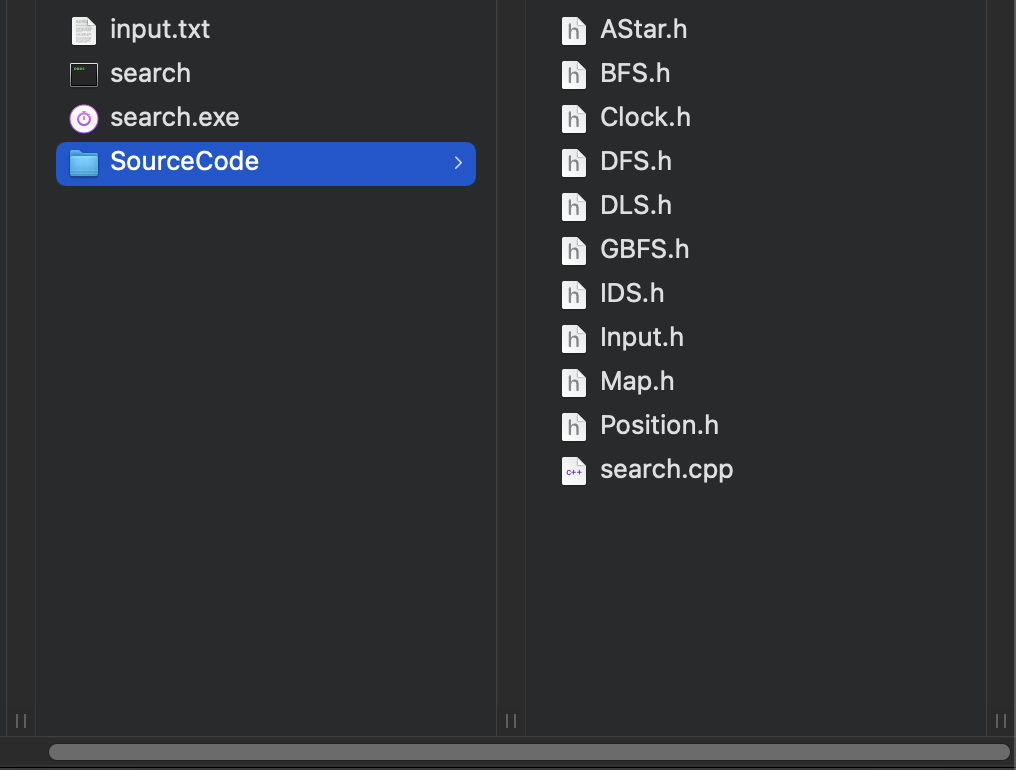
\includegraphics[width=0.7\textwidth]{./assets/FileOrganization.png}
    \caption{File Organization}
    \label{fig:fig1}
\end{figure}


\subsection{MacOS User}
For those who use MacOS systems, here is the command line to run the program on the terminal

\begin{verbatim}
Submission % ./search input.txt BFS 
\end{verbatim}

The search algorithm can be chosen by replacing ‘BFS’ with ‘DFS’, ‘GBFS’, ‘ASTAR’, and ‘IDS’. Note that if the algorithm is Iterative deepening depth-first search (IDS), the command line should be followed by the number of iterations as below 

\begin{verbatim}
Submission % ./search input.txt IDS 17 
\end{verbatim}

\subsection{Microsoft Windows 11 User}
For those who use the Microsoft Windows Operating Systems, especially Windows 11, here is the command line to run the program in the \textbf{cmd}

\begin{verbatim}
PS D:\Desktop\Submission> ./search input.txt BFS 
\end{verbatim}

\subsection{Data manipulation}
The input data may be changed by altering the \textbf{input.txt} file, but first, we must unify the Coordinate System for our Robot Navigation problem.
\subsubsection{Coordinate Systems Define}

Suppose that we have a map as below:
\begin{figure}[h]
    \centering
    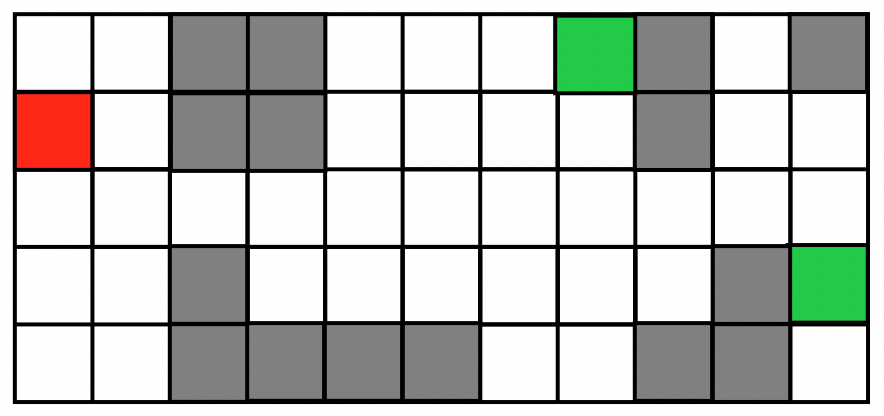
\includegraphics[width=0.6\textwidth]{./assets/Figure2.png}
    \caption{Default map}
    \label{fig:fig2}
\end{figure}

where the Red cell is the source of the Robot, the Green cell is the Destination, and the Grey cell is the obstacle/wall, which means that the Robot can not go through this cell. The position of each cell follows the rule of 2D Array, for example, in Figure \ref{fig:fig2} above, the coordinate of the Red cell is \textbf{(1, 0)}. 

Overall, given a map with width and height, the position of a cell is $(x, y)$, where $0 \leq x < \text{height}$ and $0 \leq y < \text{width.}$

\subsubsection{Data manipulation}

Here is the default \textbf{input.txt} file:
\begin{lstlisting}[caption={input.txt}]
5 11
1 0
3 10
0 2 2 2
3 2 2 1
4 3 1 3
0 8 2 1
0 10 1 1
4 8 1 1
3 9 2 1   
\end{lstlisting}

The first three lines are the basic information of the map:
\begin{itemize}
    \item The first line contains 2 integers: height and width of the map, respectively
    \item The second line contains the position of the Source of the Robot
    \item The third line contains the destination for the Robot to find out the path 
\end{itemize}

From the fourth line, each line contains 4 integers $n, m, k, q$ where $(n, m)$ is the coordinate of the leftmost top corner of a wall, $k$ and $q$ are the height and width of that wall, respectively. By following this rule, the user can modify the map in the \textbf{input.txt} file.




\section{Introduction}

Robot Navigation is one of the ideal problems in Artificial Intelligence. To solve this problem, human creates an Agent that has the ability to find out the path from a given source to the destination by 2 major searching techniques: uninformed and informed search. This report aims to explain these search methods also giving the implementation in programming language \textbf{C++}. Also, this report will cover research about the mechanism of the priority queue, which reduces the time complexity for heuristic search. 

\section{Search Algorithm and Its Implementation}
\subsection{Breadth-first Search (BFS)}
\subsubsection{BFS Idea}
In this Robot Navigation problem, the algorithm aims to explore other cells horizontally, which means that it starts visiting the source cell, then expanding its neighbor, and again, expanding the neighbors of each neighbor cell and so on until all cells are visited. To achieve this idea, the algorithm uses a queue to store the waiting cells. Frankly speaking, given a tree graph with infinite depth, the BFS algorithm can find out the goal at the $d^{th}$ depth of the graph. 
Here is the BFS pseudocode to solve our Robot Navigation problem. 

\begin{figure}[htbp]
    \centering
    \begin{mdframed}
      \begin{algorithmic}
        \STATE $cell \gets Source$
        \STATE $queue \gets $ push $cell$ to the frontier
        \STATE $visited$ visited list
        \WHILE{$queue$ is not empty}
            \STATE $currentCell \gets$ pop $queue$
            \STATE Append $currentCell$ to $visited$ 
            \FOR {$cell$ in neighbours of $currentCell$}
                \IF {$cell$ is not in $visited$}
                    \STATE $queue \gets $ push $cell$ to the $queue$
                \ENDIF
            \ENDFOR
        \ENDWHILE
      \end{algorithmic}
    \end{mdframed}
    \caption{Pseudocode for BFS algorithm}
    \label{fig:fig3}
  \end{figure}

\subsubsection{Quality}
Since the algorithm will explore cells horizontally, in other words, it will expand all the cells, therefore the algorithm requires a large amount of memory to be allocated. However, it still guarantees that it always finds the shortest path from the goal to the target.

In my implementation with the default input, the BFS algorithm takes 147,292 nanoseconds to find out the solution as Figure \ref{fig:fig4}, since our problem is simple, I decided to use nanoseconds to measure the performance, other algorithms such as DFS, GBFS, etc. will be used nanosecond to measure too. 

\begin{figure}[h]
    \centering
    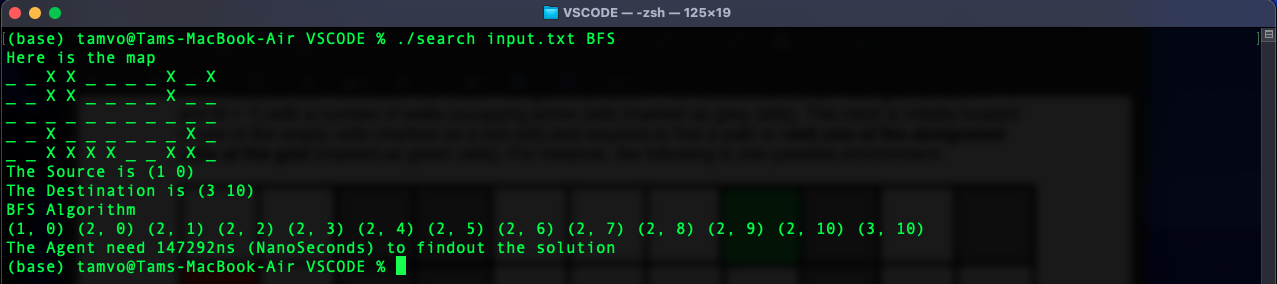
\includegraphics[width=1\textwidth]{./assets/BFS.png}
    \caption{Search result using BFS}
    \label{fig:fig4}
\end{figure}

\subsection{Depth-first Search (DFS)}
\subsubsection{DFS Idea}
The algorithm works the same as BFS, however, cells will be explored vertically, which means that it starts visiting the source, then expands a neighbor cell, and expand a neighbor of that neighbor cell, and so on until it reaches the limitation. It is easy to see that for a problem with infinite depth, DFS will never find out the solution. To achieve this idea, the algorithm uses a stack to store the waiting cells. The pseudocode to solve our problem using DFS in Figure \Ref{fig:fig5} below: 

\begin{figure}[htbp]
    \centering
    \begin{mdframed}
      \begin{algorithmic}
        \STATE $cell \gets Source$
        \STATE $stack \gets $ push $cell$ to the frontier
        \STATE $visited$ visited list
        \WHILE{$stack$ is not empty}
            \STATE $currentCell \gets$ pop $stack$
            \STATE Append $currentCell$ to $visited$ 
            \FOR {$cell$ in neighbours of $currentCell$}
                \IF {$cell$ is not in $visited$}
                    \STATE $stack \gets $ push $cell$ to the $stack$
                \ENDIF
            \ENDFOR
        \ENDWHILE
      \end{algorithmic}
    \end{mdframed}
    \caption{Pseudocode for a DFS algorithm}
    \label{fig:fig5}
 \end{figure}

\subsubsection{Quality}
As we discussed above, DFS can not return the solution for a tree graph with infinite depth. Supposed that our problem has a limited depth, DFS can find out the solution, but it does not guarantee that the solution is optimal. My implementation as Figure \Ref{fig:fig6} will prove that, although the taken time is less than BFS, the path is not optimal. 

In my perspective for this simple problem, I prefer the optimal solution rather than the taken time, so DFS is not the best choice for me.

\begin{figure}[h]
    \centering
    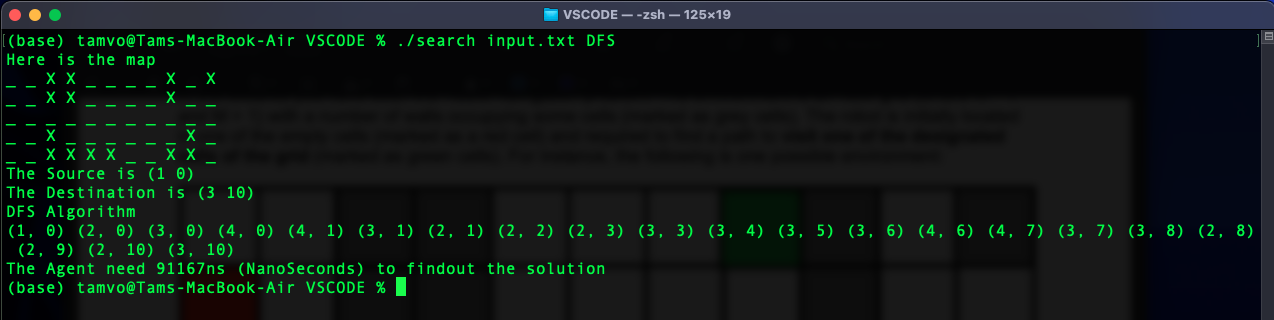
\includegraphics[width=0.8\textwidth]{./assets/DFS.png}
    \caption{Searching result using DFS}
    \label{fig:fig6}
\end{figure}

\subsection{Iterative Deepening depth-first Search (Custom Search 1)}
The Iterative Deepening depth-first Search (IDS) solves the problem of DFS: infinite depth graph, before having a deep understanding about IDS, let's take a look at Depth Limited Search (DLS)

\subsubsection{Depth Limited Search (DLS)}

The idea behind DLS is the same as DFS, however, in case it reaches the given limit depth of the graph, the algorithm will stop. Supposed the target is at level $h^{th}$, but the limitation is level $(l)^{th}$, where $l < h$, the agent will not find out the solution.

Here is the pseudocode for DLS:

\begin{figure}[htbp]
    \centering
    \begin{mdframed}
      \begin{algorithmic}
        \STATE $(cell, level) \gets (Source, 0)$
        \STATE $limit \gets$ assign limitation
        \STATE $stack \gets $ push $(cell, level)$ to the frontier
        \STATE $visited$ visited list
        \WHILE{$stack$ is not empty}
            \STATE $currentCell \gets$ pop $stack$
            \IF {$currentCell.cell$ is target}
            	\STATE return Solution
            \ENDIF
            \STATE Append $currentCell$ to $visited$ 
            \FOR {$cell$ in neighbours of $currentCell$}
            	\STATE $nextLevel \gets currentCell.level + 1$
                \IF {$cell$ is not in $visited$ and $nextLevel < limit$}
                    \STATE $stack \gets $ push $(cell, nextLevel)$ to the $stack$
                \ENDIF
            \ENDFOR
        \ENDWHILE
      \end{algorithmic}
    \end{mdframed}
    \caption{Pseudocode for DLS algorithm}
    \label{fig:fig7}
 \end{figure}
 
\subsubsection{IDS Idea}

The DLS algorithm can find out the solution as long as the limitation is greater than the depth of the target, so the IDS algorithm will try all the limitation depth from 0 to $n$, for $n \geq 0, n \in \mathbb{N}$. Here is the pseudocode for Iteravite Deepening depth-first Search:

\begin{figure}[htbp]
    \centering
    \begin{mdframed}
      \begin{algorithmic}
        \STATE $limitation \gets$ assign limitation
        \FOR {limit in range(0, limitation)}
        	\STATE $DLS$(graph, target, source , limit)
        \ENDFOR
      \end{algorithmic}
    \end{mdframed}
    \caption{Pseudocode for IDS algorithm}
    \label{fig:fig8}
 \end{figure}
 
\subsubsection{Quality}

The solution is based on the idea of DFS, so it is not optimal. Plus, the algorithm still depends on a factor: the number of iterations, or the limitation. As Figure \ref{fig:fig9} below, with 12 iterations, the path can not be found:

\begin{figure}[h]
    \centering
    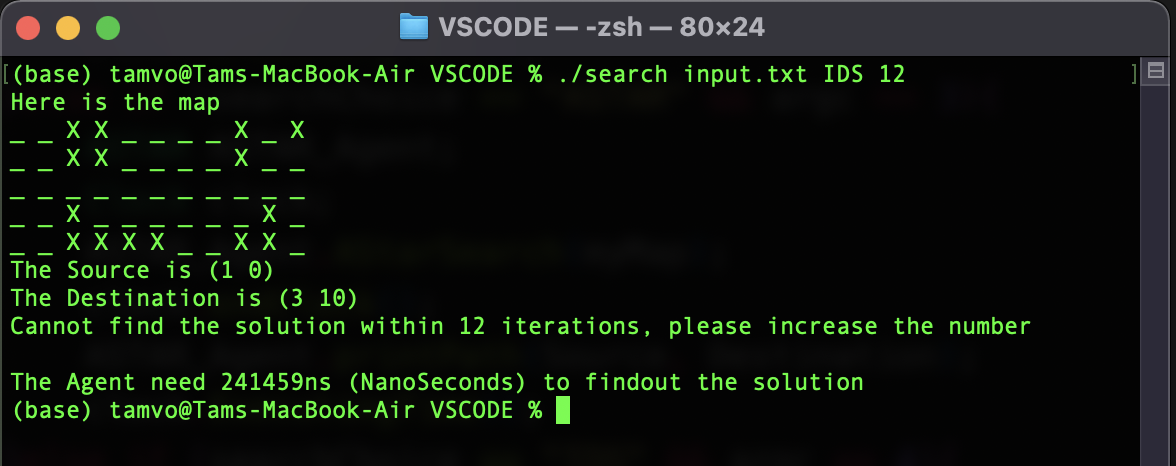
\includegraphics[width=0.8\textwidth]{./assets/IDS1.png}
    \caption{Searching result using IDS with 12 iterations}
    \label{fig:fig9}
\end{figure}

Now this is the terrible result after increasing the iteration to 25:

\begin{figure}[h]
    \centering
    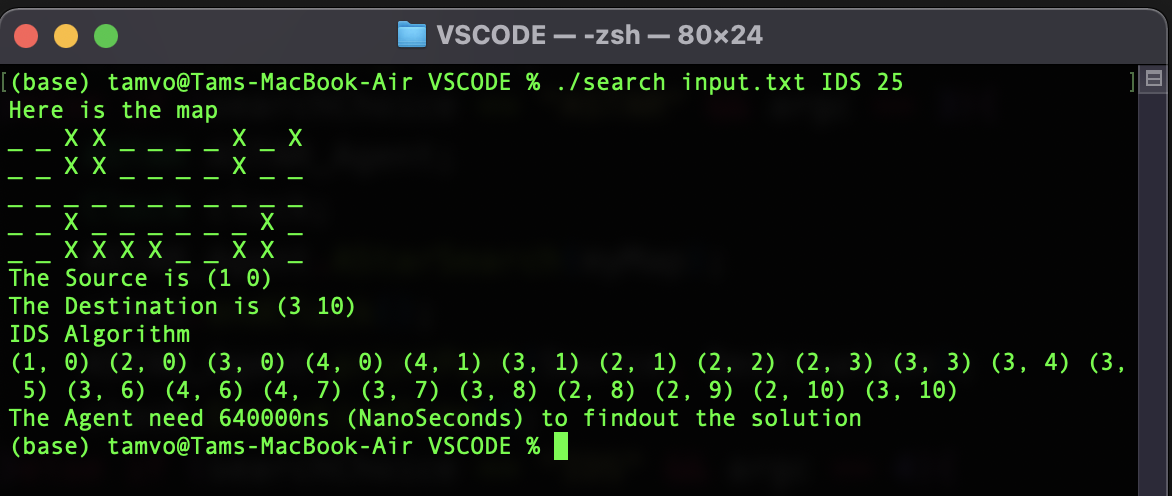
\includegraphics[width=0.8\textwidth]{./assets/IDS2.png}
    \caption{Searching result using IDS with 12 iterations}
    \label{fig:fig10}
\end{figure}

With those uninformed search techniques above, I prefer BFS algorithm to find out the solution despite its costly space required. 

\subsection{Greedy Best-first Search (GBFS)}

\subsubsection{Idea}
The idea of GBFS is the same as BFS, however, instead of using a queue to store the waiting cells, the algorithm uses a priority queue and a heuristic function $h(x)$ to evaluate the current cell. In our Robot Navigation problem, the heuristic function is the Manhattan method. Below is the Manhattan method which takes the positions of two cells: the current cell and the goal cell:

\begin{lstlisting}[caption={Manhattan Function in C++}]
#include <iostream>
using namepace std;

int Manhattan(Position x, Postion Goal){
	return (abs(x.row - Goal.row) + abs(x.col - Goal.col));
}
\end{lstlisting}

For example, supposed the current cell is $(1, 0)$ and our goal is $(3, 10)$. The next cells that will be explored are $(0, 0)$, $(2, 0)$, and $(1, 1)$, by passing them to the Manhattan heuristic function, the values we will get are $13$,$11$, and $11$, respectively. Next, we push cells $(0, 0)$, $(2, 0)$, and $(1, 1)$ to the priority queue, if we pop a cell from the queue above, we can get $(1, 1)$ or $(2, 0)$ because it seems that those cells are closer to the goal and more potential to find the path.

Here is the pseudocode for GBFS:

\begin{figure}[htbp]
    \centering
    \begin{mdframed}
      \begin{algorithmic}
        \STATE $cell \gets Source$
        \STATE $priotityQueue \gets $ push $cell$ to the frontier
        \STATE $visited$ visited list
        \WHILE{$priorityQueue$ is not empty}
            \STATE $currentCell \gets$ pop $priorityQueue$
            \IF {$currentCell$ is goal}
            	\STATE return solution
            \ENDIF
            \STATE Append $currentCell$ to $visited$ 
            \FOR {$cell$ in neighbours of $currentCell$}
                \IF {$cell$ is not in $visited$}
                    \STATE $priotiyQueue \gets $ push $cell$ to the $priorityQueue$
                \ENDIF
            \ENDFOR
        \ENDWHILE
      \end{algorithmic}
    \end{mdframed}
    \caption{Pseudocode for GBFS algorithm}
    \label{fig:fig11}
 \end{figure}

\subsubsection{Quality}

GBFS algorithm performance depends on the heuristic function, we can use the Euclidean method as a heuristic function but it is not optimal as the Manhattan method. My result after using GBFS to find the solution is in Figure \ref{fig:fig12}, the result is better than other search methods. 

\begin{figure}[h]
    \centering
    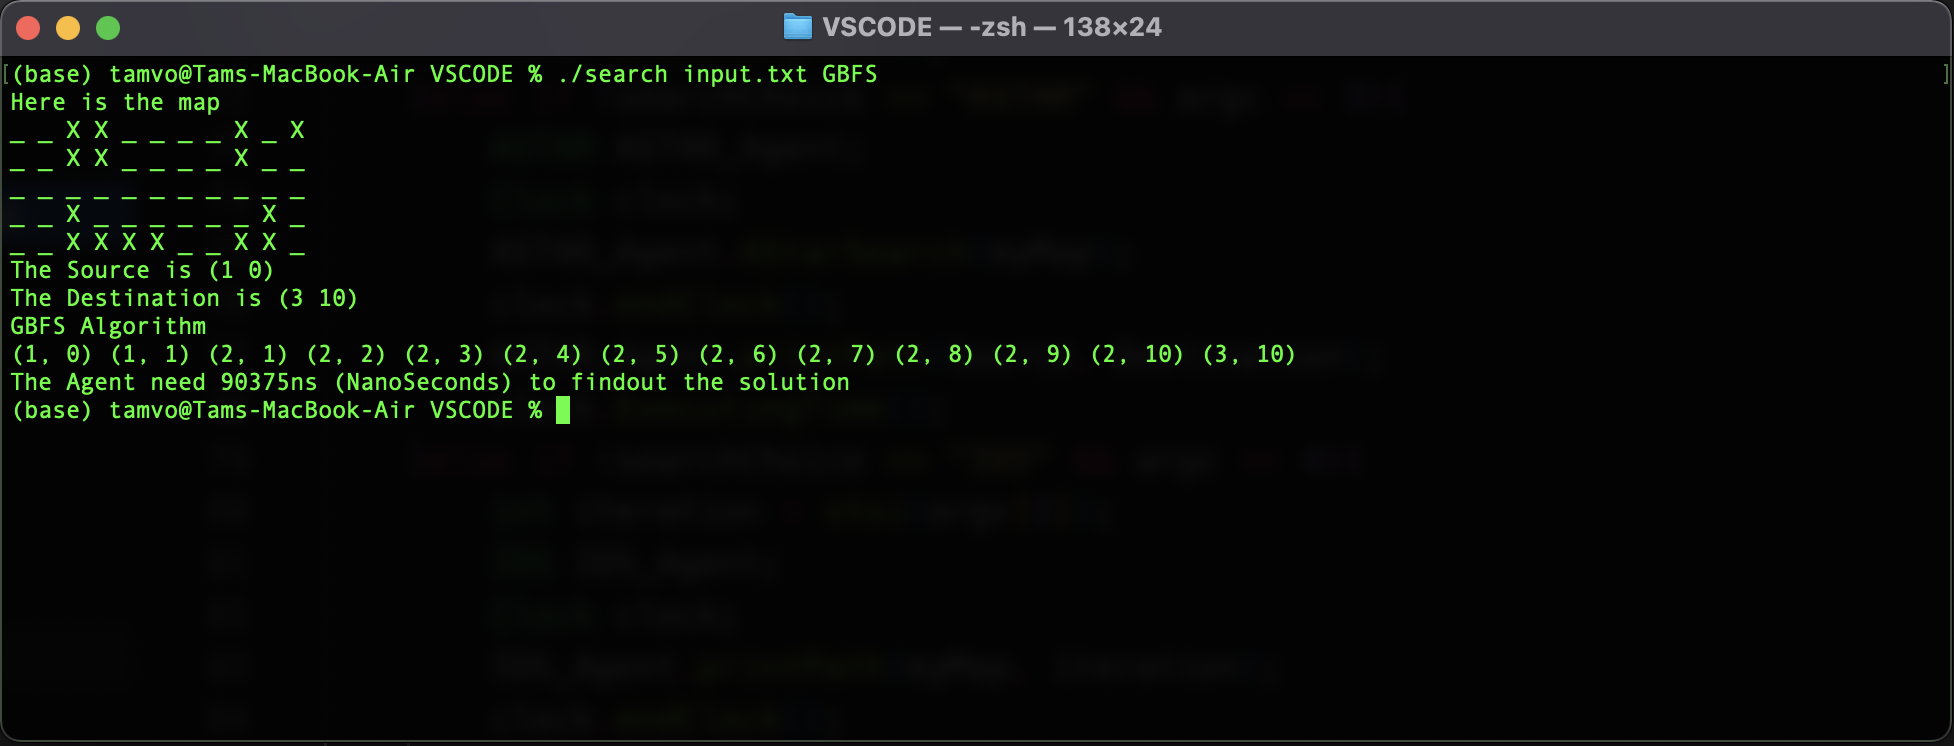
\includegraphics[width=1\textwidth]{./assets/GBFS.png}
    \caption{Searching result using GBFS}
    \label{fig:fig12}
\end{figure}

It seems that the agent will quickly find out the solution with a heuristic search, although the path is not better than BFS, which always gives the optimal path, the performance of GBFS is still impressive. 

\subsection{A* Search}

\subsubsection{Idea}
A* Algorithm is also based on the GBFS, however instead of using only the $h(x)$ function to evaluate the potential of the cell, A* combines $g(x) + h(x)$, where $g(x)$ is the actual distance from the source to the checking cell. A good heuristic function in A* star is called "Admissible", which means that it never overestimates the cost to reach the goal. Pseudocode for A* Search will not be shown here because it is the same as GBFS but uses a different evaluation function.

\subsubsection{Quality}

In our problem, the distance between two adjacent cells is always 1, therefore, A* Searching will not return the optimal solution to find the path, although the executing time is less than other uninformed searches. Here is my result after implementing this searching technique:

\begin{figure}[h]
    \centering
    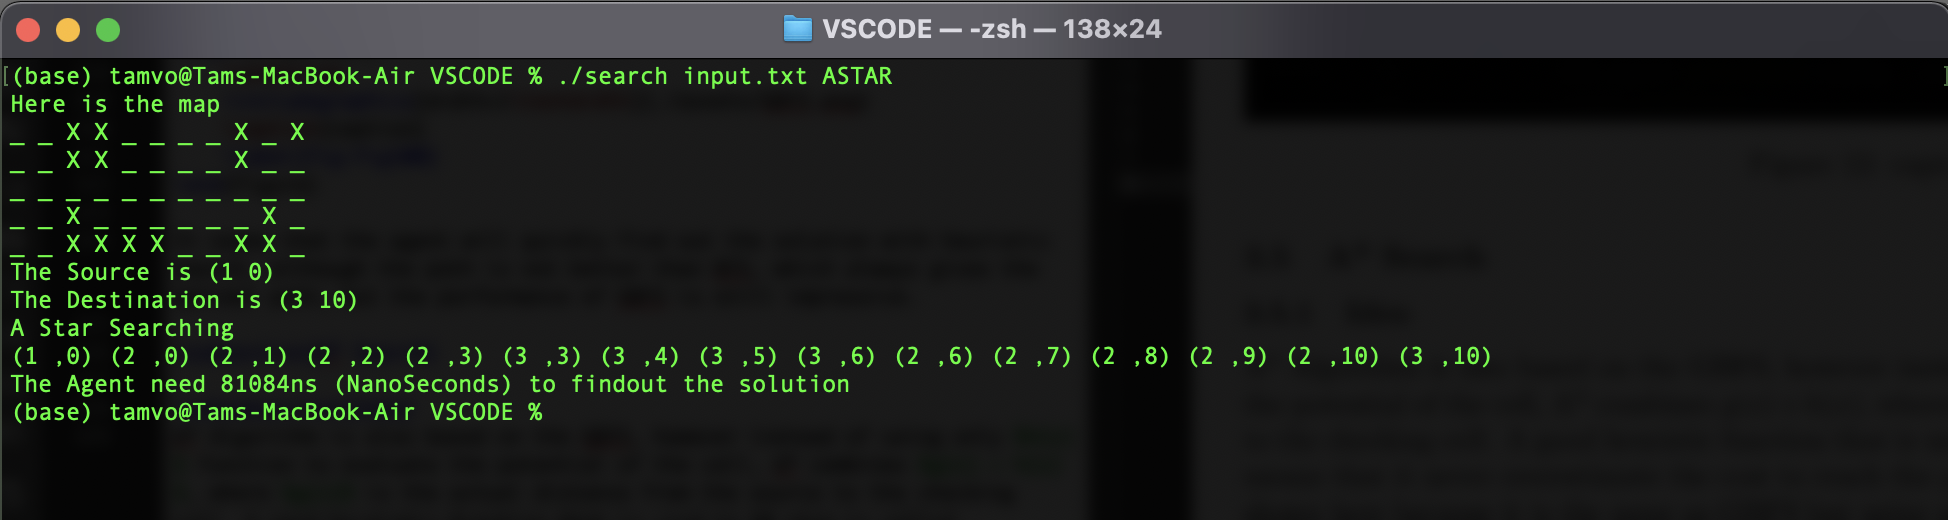
\includegraphics[width=1\textwidth]{./assets/ASTAR.png}
    \caption{Searching result using A* }
    \label{fig:fig13}
\end{figure}

\newpage
\section{Programming Overview Design}
The UML diagram below demonstrates the relationship in the program. There are 11 classes. This section will not explain the function of these classes: BFS, DFS, GBFS, ASTAR, IDS, and DLS because obviously, they are in charge of searching the path. Meanwhile, 

\begin{itemize}
  \item Input class is responsible for reading data from \textbf{input.txt}
  \item Clock class is responsible for measuring the performance of a searching technique
  \item Map class is responsible for storing information about the environment
\end{itemize} 

Here is the UML diagram:
\begin{figure}[h]
    \centering
    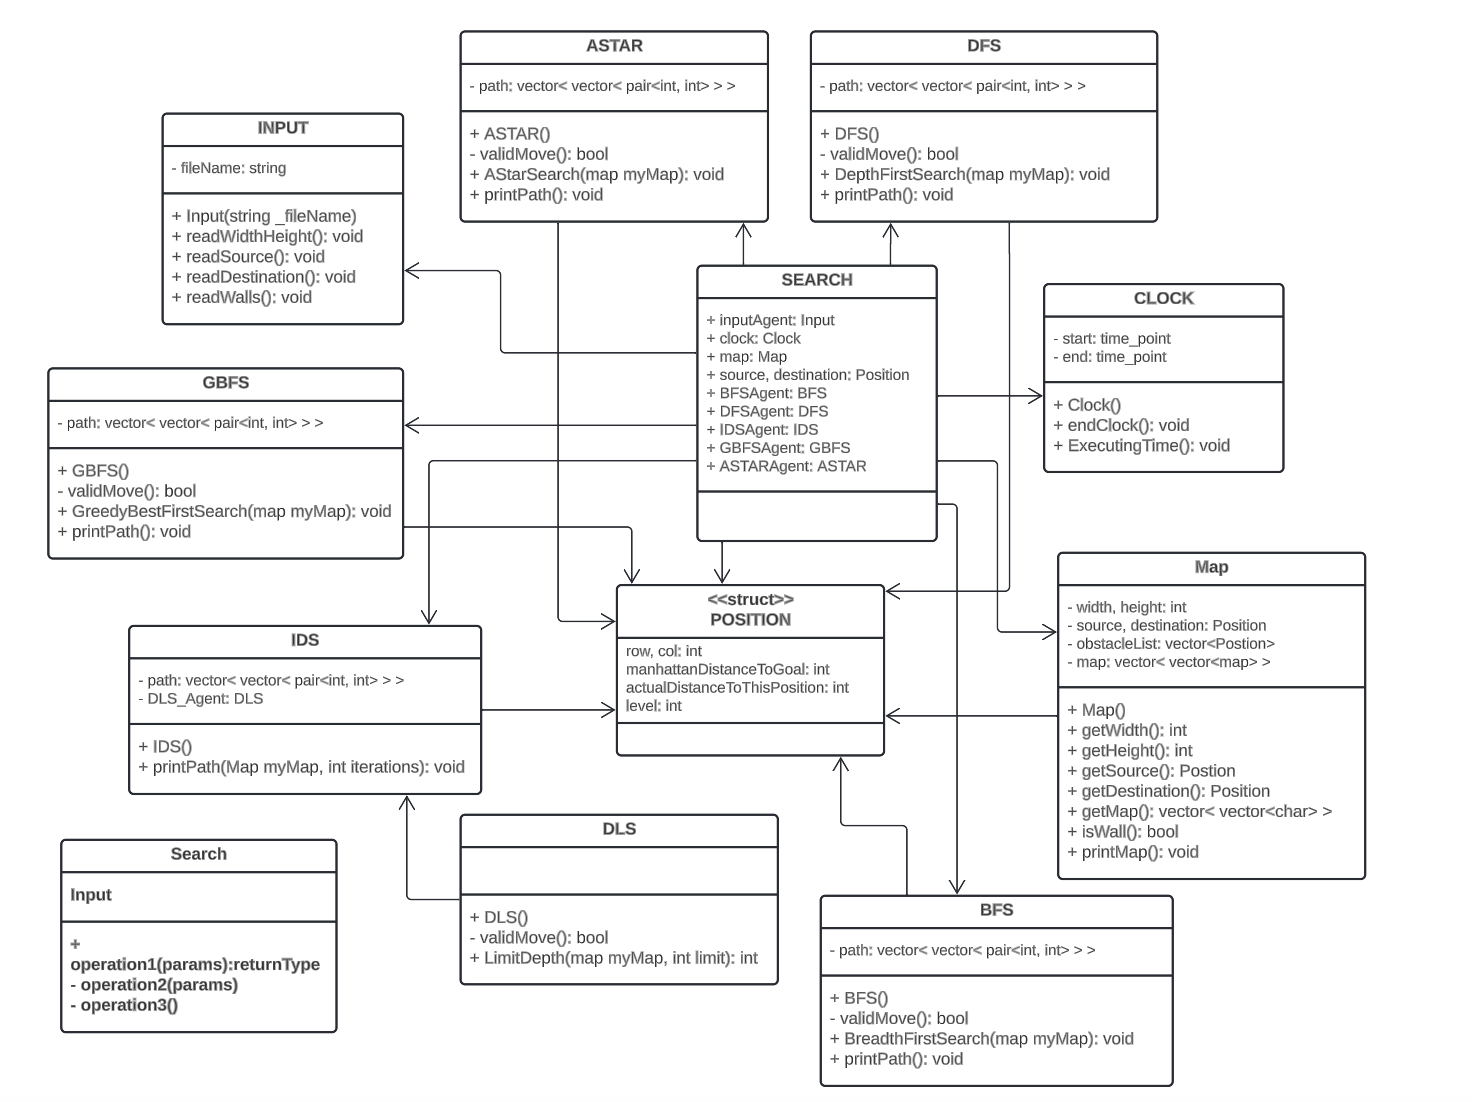
\includegraphics[width=1\textwidth]{./assets/UML.png}
    \caption{UML Diagram}
    \label{fig:fig14}
\end{figure}

\newpage
\section{Research field: Mechanism Behind Priority Queue}
\subsection{Introduction}
In informed search implementation, the main difference is the frontier, instead of using a queue or stack to store the waiting cells, the priority queue is chosen to reduce the time complexity. The priority queue allows getting the maximum or minimum element with time complexity $O(1)$ and pushing/popping an element with the time complexity $O(logN)$. The idea behind the priority queue is based on the Heap data structure, which will be discovered in this session.
\subsection{Heap Data Structure Overview}
There are two types of Heap: Min Heap and Max Heap. The implementation of this program is prioritizing the cell with the lowest Manhattan Distance to the Goal, so Min Heap will be the main topic to be discussed. Below is one of the implementations of the priority queue in the program:

\begin{lstlisting}[caption={Using priority queue in program}]
#include <iostream>
#include <queue>
#include <vector>
using namepace std;
class GBFS{
	/// code
		
	void GreedyBestFirstSearch(Map myMap){
	/// declare the built-in priority queue
    priority_queue< Position, vector<Position>, optionManhattan > frontier;
    
    /// code
	}
};
\end{lstlisting}

\subsubsection{Properties}
First, Min Heap is a complete binary tree, whose nodes at each level (except the level containing leaf nodes or the lowest level) are always fully filled. At the lowest level, leaf nodes should be filled from the left-hand side. Figure \ref{fig:fig15} below shows the demonstration of a complete binary tree:

\begin{figure}[h]
    \centering
    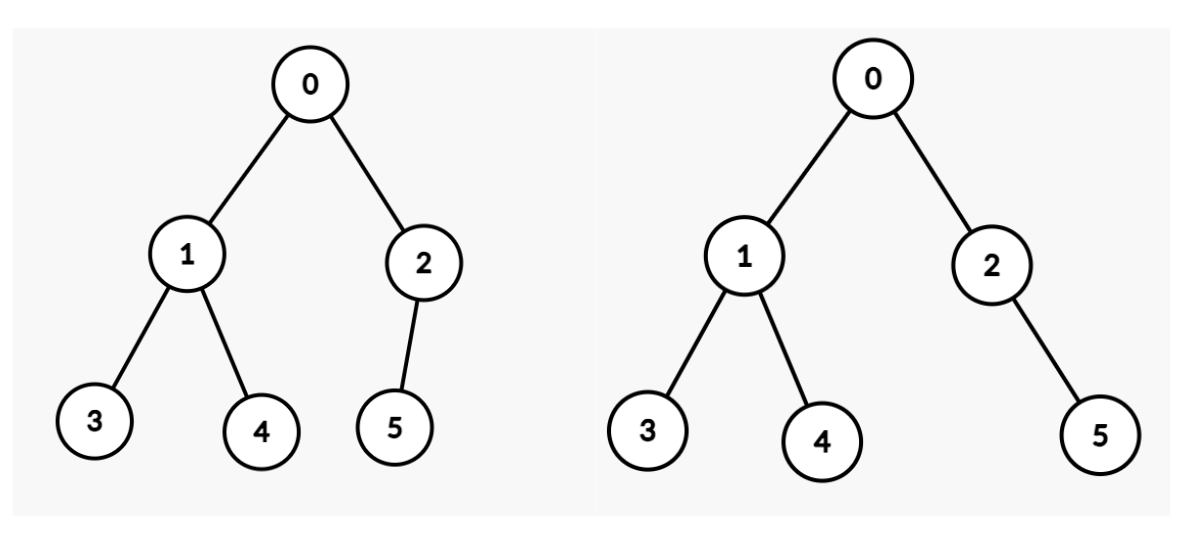
\includegraphics[width=0.7\textwidth]{./assets/completeBinaryTree.png}
    \caption{Complete Binary Tree and Incomplete Binary Tree}
    \label{fig:fig15}
\end{figure}

Second, in Mean Heap, the root is always the smallest element and every parent node is always less than its child nodes as Figure \ref{fig:fig16} below:

\begin{figure}[h]
    \centering
    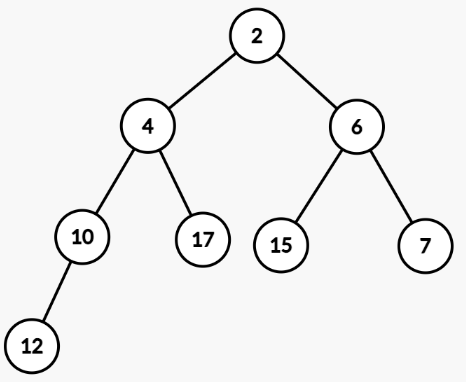
\includegraphics[width=0.5\textwidth]{./assets/MinHeapEx.png}
    \caption{Example of a Min Heap}
    \label{fig:fig15}
\end{figure}

\subsubsection{Using array to present Min Heap Data structure}
We can use an array to present the Heap data structure: the first element at index 0 is always the root of the binary tree, and its child nodes are at index 1 and 2. Following that, the child nodes of index 1 are at 3 and 4, and so on. Hence we have:

Given an index $a$, its child nodes are at $(2a + 1)$ and $(2a + 2)$. 

For example, Figure \ref{fig:fig16} below is a array representation for the Min Heap in Figure \ref{fig:fig15}

\begin{figure}[h]
    \centering
    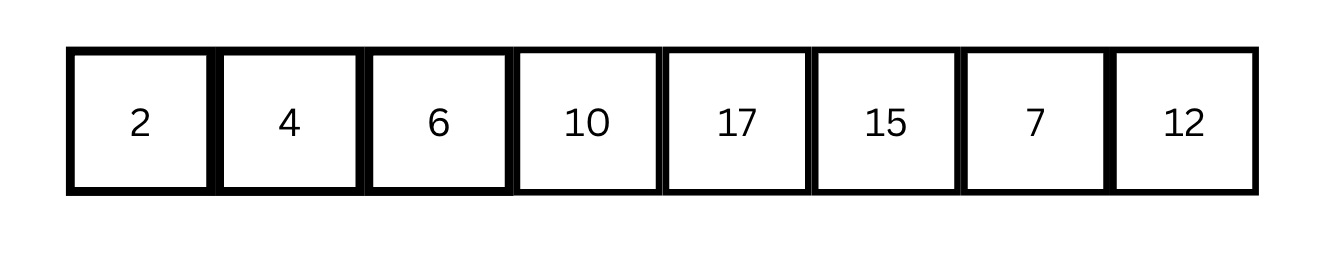
\includegraphics[width=0.6\textwidth]{./assets/exArray.png}
    \caption{Array representation for Figure \ref{fig:fig15}}
    \label{fig:fig16}
\end{figure}


\subsection{Min Heap Operation}
There are 3 main operations that we can interact with a Min Heap including Heapify, Insertion, and Deletion.

\newpage
\subsubsection{Heapify}
Heapify is an action that converts a normal array into a heap data structure. Beginning with the last node that has the leaf, then we check and swap its order with its child nodes’ order in the array.

Here is the pseudocode for Heapify 

\begin{figure}[htbp]
    \centering
    \begin{mdframed}
      \begin{algorithmic}
    \STATE \textbf{Function} \textit{Heapify}(index, array)
	\STATE \hspace*{0.5cm} // Calculates the sum of two numbers 
	\STATE \hspace*{0.5cm} current = index
	\STATE \hspace*{0.5cm} leftChild = 2 * index + 1
	\STATE \hspace*{0.5cm} rightChild = 2 * index + 2
		
	\STATE \hspace*{0.5cm} // Swap current position with its left child node
	\STATE \hspace*{0.5cm} \textbf{if} leftChild $<$ size of array \textbf{and} array[leftChild] $<$ array[current] \textbf{then}
		\STATE \hspace*{1cm} current = leftChild
	\STATE \hspace*{0.5cm} \textbf{end if}
	
	\STATE \hspace*{0.5cm} // Swap current position with its right child node
	\STATE \hspace*{0.5cm} \textbf{if} rightChild $<$ size of array \textbf{and} array[rightChild] $<$ array[current] \textbf{then}
		\STATE \hspace*{1cm} current = rightChild
	\STATE \hspace*{0.5cm} \textbf{end if}
	
	\STATE \hspace*{0.5cm} // Recursively checking
	\STATE \hspace*{0.5cm} \textbf{if} current $!=$ index \textbf{then}
		\STATE \hspace*{1cm} swap(array[current], array[index])
		\STATE \hspace*{1cm} \textit{Heapify}(current, array)
	\STATE \hspace*{0.5cm} \textbf{end if}
	\STATE
\STATE \textbf{Function} \textit{HeapifyArray} (array)
	\STATE \hspace*{0.5cm} \textbf{for} i = size of array / 2 - 1; i $\geq$ 0; i-- \textbf{do}
		\STATE \hspace*{1cm} \textit{Heapify} (i, array)
	\STATE \hspace*{0.5cm} \textbf{end for}
\end{algorithmic}
    \end{mdframed}
    \caption{Pseudocode for Heapify an array}
    \label{fig:fig18}
 \end{figure}
 
The algorithm above has a time complexity of $O(logN)$ and the space complexity is $O(N)$.

\newpage
\subsubsection{Insertion}

Given a min heap array, adding a new element is pushing back that element at the end of the array, then we modify its position in the array to satisfy the requirement of a heap data structure. This operation is easy to understand because we do not need to use recursion to do it. Here is the pseudocode for inserting an element into a heap array:

\begin{figure}[htbp]
    \centering
    \begin{mdframed}
      \begin{algorithmic}
    \STATE \textbf{Function} \textit{insert}(element, array)
	\STATE \hspace*{0.5cm} // Pushing back the element at the end of the array
	\STATE \hspace*{0.5cm} array $\gets$ pushing back element
	\STATE \hspace*{0.5cm} currentIndex $\gets$ size of array - 1	
	
	\STATE
	\STATE \hspace*{0.5cm} \textbf{While} cuurrentIndex != 0 \textbf{and} array[(currentIndex - 1) / 2] $>$ array[currentIndex] \textbf{do}
	\STATE \hspace*{1cm} swap(array[(currentIndex - 1) / 2], array[currentIndex])
	\STATE \hspace*{1cm} currentIndex = (currentIndex - 1) / 2
	\STATE \hspace*{0.5cm} \textbf{end while}  \textbf{do}
\end{algorithmic}
    \end{mdframed}
    \caption{Pseudocode for inserting an element to a heap}
    \label{fig:fig20}
 \end{figure}

The algorithm above has a time complexity of $O(logN)$ and the space complexity is $O(N)$.


\subsubsection{Deletion}
Deletion of an element of a heap array is deleting the root of the binary tree or the first element of the array. then we must heapify the array again to adapt the rule of array representation for Heap. The idea is to replace the first element with the last element, next, we delete the last element and heapify the array from the first position. 

Here is the Pseudocode for deleting an element of a heap data structure:
\begin{figure}[htbp]
    \centering
    \begin{mdframed}
      \begin{algorithmic}
    \STATE \textbf{Function} \textit{delete}(array)
	\STATE \hspace*{0.5cm} // Pushing back the element at the end of the array
	\STATE \hspace*{0.5cm} Swap the first element and the last element
	\STATE \hspace*{0.5cm} Delete the last element of the array
	\STATE \hspace*{0.5cm} \textit{Heapify}(0, array)
\end{algorithmic}
    \end{mdframed}
    \caption{Pseudocode for deleting an element from a heap}
    \label{fig:fig21}
 \end{figure}
 
 The algorithm above has a time complexity of $O(logN)$ and the space complexity is $O(N)$.
 
\subsection{Conclusion}
Instead of sorting the queue to get the smallest element, by implementing the priority queue in informed searching, the time complexity is reduced significantly. Therefore, the performance of the Agent will be more impressive. 

\section{Reference}
\bibitem{CLRS09}
Cormen, T. H., Leiserson, C. E., Rivest, R. L., & Stein, C. (2009). \textit{Introduction to Algorithms} (3rd ed.). MIT Press.
\end{document}

